\documentclass[pdf]{beamer}
\usepackage[latin1]{inputenc}
\usepackage{multirow}
\usetheme{Warsaw} %Warsaw
\usecolortheme{seahorse}


\begin{document}

\title[RNAseq]{RNAseq}
\subtitle{BCB 504: Applied Bioinformatics\\}
\author[Matt Settles]{Matt Settles}
\institute{University of Idaho\\ Bioinformatics and Computational Biology Program}
\date{\today}


%% Title page
\begin{frame}[plain]
  \titlepage
\end{frame}


%% Outline
\begin{frame}[plain] 
  \frametitle{Outline}
  \tableofcontents
\end{frame}

\section{Introduction}
\begin{frame}
  \frametitle{Inroduction}
\centering\alert{RNA-Seq: a revolutionary tool for transcriptomics}
\begin{center}
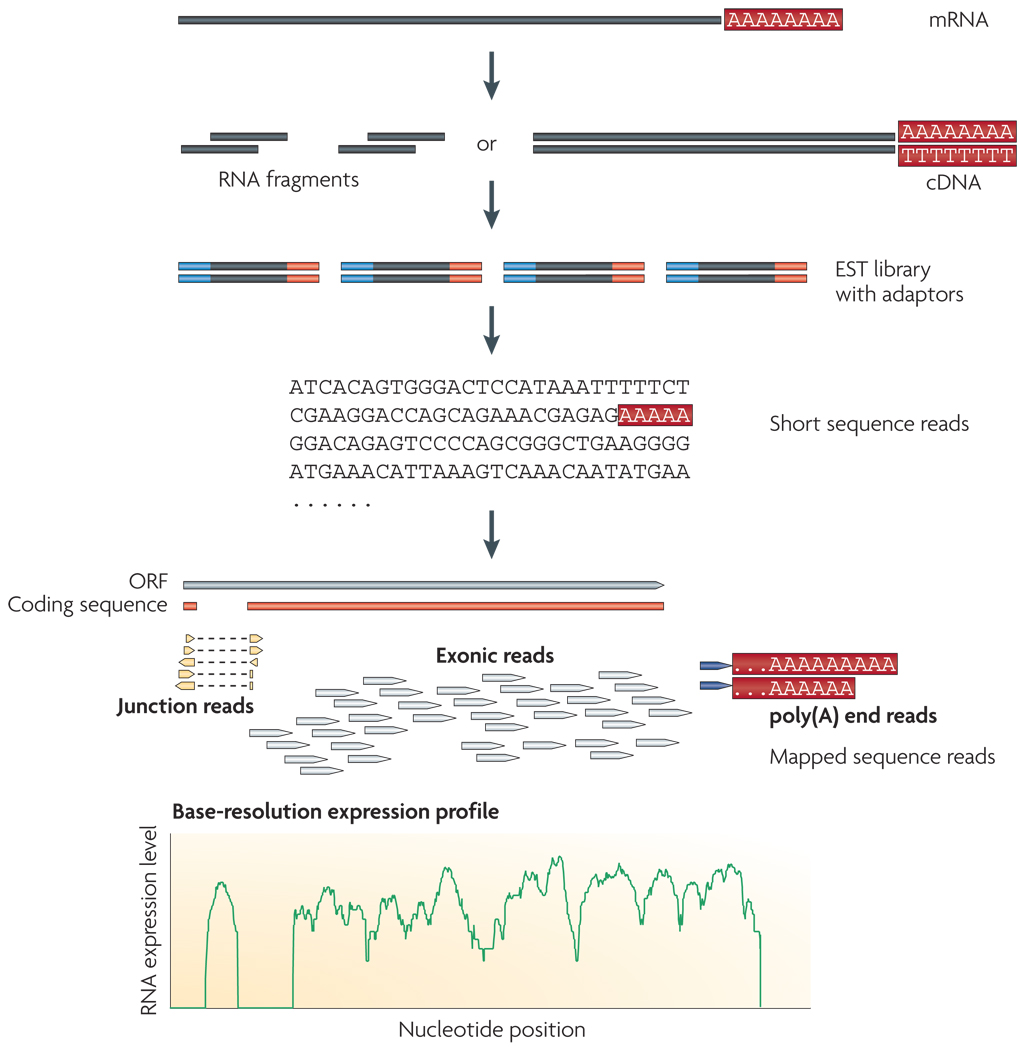
\includegraphics[scale=0.35]{Figures/nihms229948f1.jpg} 
\end{center}
\end{frame}

\section{RNA-seq mapping}

\begin{frame}
\frametitle{RNA-seq Junction Mapping}
\alert{In RNA-seq data, you must also map splice junctions, reads may span an intron}
\begin{center}
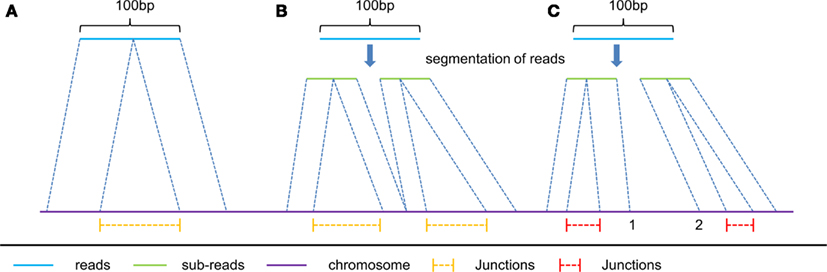
\includegraphics[scale=0.4]{Figures/junctions.jpg} 
\end{center}
\end{frame}

\begin{frame}
\frametitle{Some algorithms}
\begin{itemize}
\item Tophat (Bowtie2)
\item SOAPsplice
\item SPLICEmap
\item TrueSite
\end{itemize}
\end{frame}


\section{de novo RNA assembly}
\begin{frame}
\frametitle{Splice Variation}
Ambiguities in transcriptome assembly contigs usually correspond to spliced isoforms, or minor variation among members of a gene family.
\begin{center}
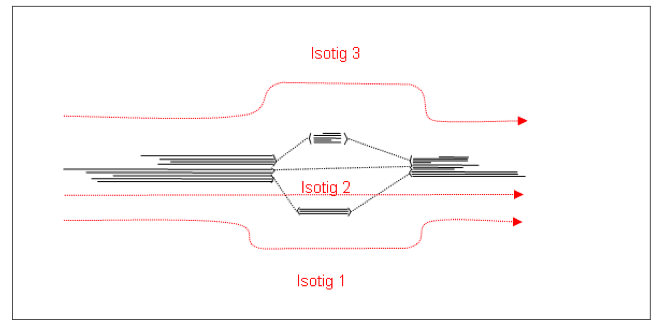
\includegraphics[scale=0.4]{Figures/spliceVariation.png} 
\end{center}
\end{frame}
\subsection{Trinity}

\begin{frame}
  \frametitle{Trinity}
  \begin{description}
    \item [Inchworm] assembles the RNA-Seq data into transcript sequences, often generating full-length transcripts for a dominant isoform, but then reports just the unique portions of alternatively spliced transcripts.
    \item [Chrysalis] clusters the Inchworm contigs and constructs complete de Bruijn graphs for each cluster. Each cluster represents the full transcriptional complexity for a given gene (or a family or set of genes that share a conserved sequence). Chrysalis then partitions the full read set among these separate graphs.
    \item [Butterfly] then processes the individual graphs in parallel, tracing the paths of reads within the graph, ultimately reporting full-length transcripts for alternatively spliced isoforms, and teasing apart transcripts that corresponds to paralogous genes.
  \end{description}
\end{frame}

\begin{frame}
  \frametitle{Trinity}
  \begin{center}
  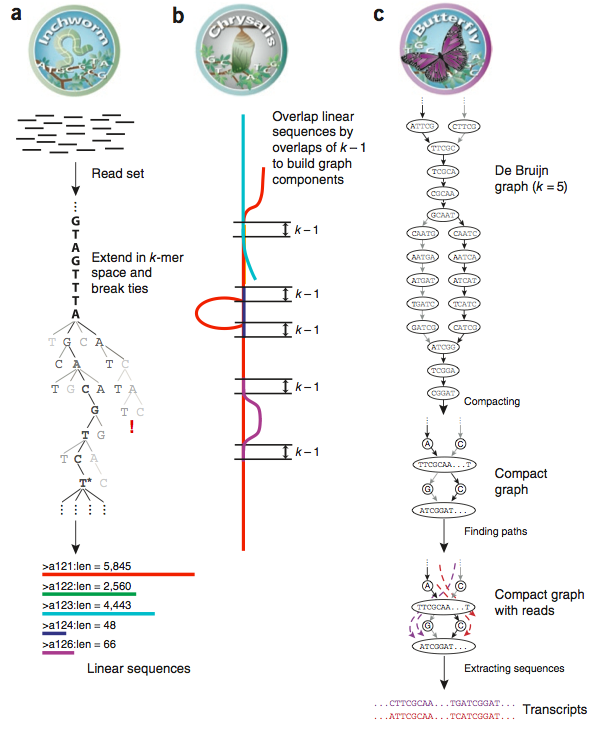
\includegraphics[scale=.25]{Figures/trinity.png} 
  \end{center}
\end{frame}

\subsection{Newbler}
\begin{frame}
  \frametitle{Newbler}
  Isotig (isoform) initiation:
  \begin{itemize}
    \item Contigs lacking reads connecting them to other contigs on one or both ends are used to initiate the traversal of an individual isotig. When a contig has no reads connecting it to any other contigs, it may become an isotig composed of a single contig.
    \item Spike detection
    \begin{enumerate}
    \item The alignment depth is at least 10 reads.
    \item A minimum of 20\% of the aligned reads must be in the opposite orientation relative to the more abundant orientation of the aligned reads.
    \item A spike may not occur within 10 bases of an already detected spike.
    \item A change in alignment depth between one alignment column and the next of at least 50\% signals the location of a "spike".
    \end{enumerate}
  \end{itemize}
\end{frame}

\begin{frame}[allowframebreaks]
  \frametitle{Newbler}
  Isotig (isoform) extension is then done by following reads that join together contigs. Finally, isotigs are terminated by one of the following conditions:
  \begin{enumerate}
  \item No reads are found that extend from the contig currently at the end of the isotig path.
  \item The number of reads connecting two contigs is less than 5\% of the alignment depth of either.
  \item The Isotig Contig Count Threshold is reached. In this case, the further traversal of a particular isotig in an isogroup will be stopped.
  \item A contig is reached whose length is below the Isotig Contig Length Threshold. If a contig is reached with a length shorter than this threshold, the further traversal of a particular isotig in an isogroup will be stopped. The contig shorter than the icl threshold will be marked as such and reported in the output files.
  \item A cyclic path is encountered. Recursive path traversal will stop if cyclic structures are detected, i.e. revisiting one contig which has already been included in an earlier part of the isotig being traversed. Such cyclic structures will be marked in the output files by assigning cyclic status for the first contig detected.
  \end{enumerate}
\end{frame}

\subsection{Fusion transcripts}
\begin{frame}
  \frametitle{Fusion transcripts}
  Fusion transcript is a chimeric RNA encoded by a fusion gene or by two different genes by subsequent trans-splicing. Certain fusion transcripts are commonly produced by cancer cells, and detection of fusion transcripts is part of routine diagnostics of certain cancer types.
  \begin{center}
  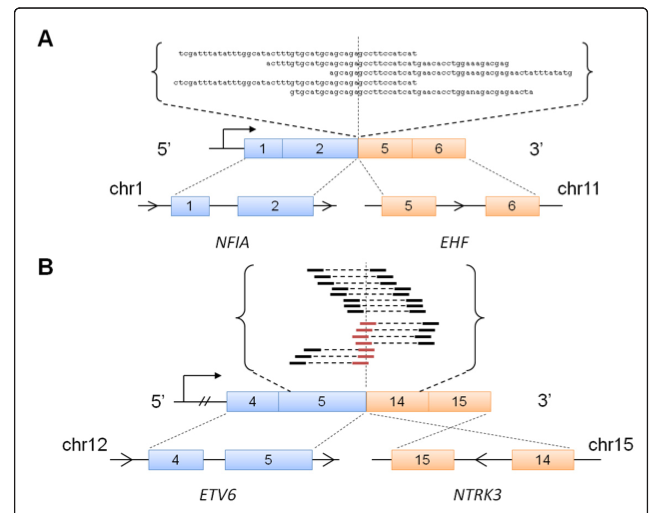
\includegraphics[scale=0.22]{Figures/fusion.png} 
  \end{center}
\end{frame}

%\section{RNA mapping}
%\begin{frame}
%  \frametitle{Gapped Alignment}
%  Problem: Burrows-Wheeler transform (BWT) facilitate very efficient ungapped alignment of short reads.\\
%   Gaps greatly increase the size of the search space and reduce the effectiveness of pruning, thereby substantially slowing aligners built solely on index-assisted alignment.\\
%\vspace{0.2in}
%  For RNA, aligners must be able to produce gapped alignments, reads are expected to span introns.
 % \begin{itemize}
 % \item BarraCUDA
 % \item BWA
 % \item gMAP (gSNAP)
 % \item Mosaik
 % \item Novoalign
 % \item tophat/cufflinks extension to bowtie
 % \end{itemize}
  
%\end{frame}

\section{Digital Transcriptomics}
\begin{frame}
  \frametitle{Digital Transcriptomics}
The more you can count - and next-generation systems can count a lot - the better the measure of copy number for even those rare transcripts in a population.\\
\vspace{0.2in}
  \begin{itemize}
   \item Most techniques deal with Count data. Reads are mapped to a reference genome, transcripts are detectd, and the number of reads that map to a trascript (or gene) and counted.
  \item Read counts for a transcript are roughly proportional to the gene's length and transcript abundance.
  \item technical artifacts then must be considered and the data normalized
  \begin{itemize}
    \item the sample depth of sequencing
    \item GC count (PCR type bias)
    \item mappability (uniqueness)
  \end{itemize}  
  \end{itemize}
\end{frame}

\begin{frame}
  \frametitle{Digital Transcriptomics}
  \begin{itemize}
  \item Differential Expression between phenotypes is then determined from the count data.
  \item Count data is modeled by a discribution (ie. Negative Bionomial Distribution, Poisson, etc.)
  \item Generally speaking differential expression analysis is performed in a very similar manner to DNA microarrays, once bias and normalization have  been performed.
  \end{itemize}
\end{frame}

\begin{frame}
\frametitle{RPKM and FPKM}
\textbf{RPKM} - Reads per kilobase per million mapped reads\\
\vspace{0.4in}
\textbf{FPKM} - Fragments per kilobase per million mapped reads\\
\end{frame}

\begin{frame}
\frametitle{Analysis packages}
A lot of RNA-seq analysis has been done in R and so there are many packages available to analyze and view this data. Two of the best are:\\
\begin{itemize}
\item DEseq
\item edgeR (extension to Limma [microarrays] for RNA-seq)
\end{itemize}
\vspace{0.2in}
\url{http://www.bioconductor.org/packages/release/BiocViews.html\#___RNAseq}
\end{frame}

\begin{frame}
\frametitle{Bowtie2, Tophat, Cufflinks, CummeRbund Pipeline}
\begin{itemize}
\item \textbf{cufflinks}
\begin{itemize}
\item cufflinks assembles each transcript from the Tophat mapping results
\end{itemize}
\item \textbf{cuffcompare}
\begin{itemize}
\item cuffcompare compares your assembled results to a reference file (gff or gtf), and/or across experiments
\end{itemize}
\item \textbf{cuffmerge}
\begin{itemize}
\item cuffmerge merges assembled results across multiple samples, determines 'comparable' transcripts across samples.
\end{itemize}
\item \textbf{cuffdiff}
\begin{itemize}
\item cuffdiff computes significant changes in transcript expression, splicing, and promoter use.
\end{itemize}
\end{itemize}
\end{frame}

\begin{frame}
\frametitle{How cuffdiff finds differential transcripts}
\begin{center}
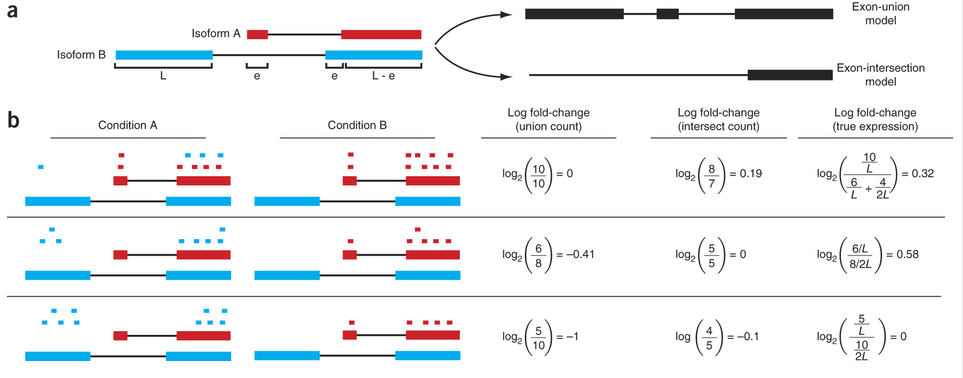
\includegraphics[scale=0.35]{Figures/cuffdiff.png} 
\end{center}
\end{frame}

\end{document}

